\chapter{Conclusion}

What, then, has our body of work, as well as the numerous other recent investigations into mergers and post-merger evolution, taught us about the fate of sub-\Mch\ CO WD mergers?  Are there systems that compress and heat enough during post-merger evolution to ignite degenerate carbon burning near their centers, which then leads to an explosion?  Below, I summarize our current understanding of these systems and the sub-\Mch\ merger channel scenario proposed by \citeal{vkercj10}, and suggest avenues for future exploration.

\section{Mergers and Early Post-Merger Evolution}

In Ch. \ref{ch:ch2}, we used SPH simulations of double CO WD mergers to explore the range of possible merger remnants and determine which among them are candidates for ignition under highly degenerate conditions during post-merger evolution.  The properties most important for this are the temperature and degree of rotational support of the dense remnant core, and we find that dissimilar-mass mergers result in cold and slowly-rotating cores that are unlikely to subsequently ignite, while similar-mass ones have cores that are heated abnd partly rotationally supported throughout.  The (rough) dividing line between the two classes is a density ratio between donor and accretor WD of $\qrho\simeq0.6$, equivalently a difference between their masses of $\Delta M \simeq 0.1\,\Msun$.

Since the publication of Ch. \ref{ch:ch2}, \cite{dan+14} published their study of remnants from synchronized WD mergers with exact initial conditions.  They find that for all of their merger remnants -- even ones we deem similar-mass -- the mass enclosed within the radius of maximum temperature \MencTmax\ is approximately the mass of the accreting WD, and the temperature at the remnant's center is a factor of at least a few lower.  Their similar-mass mergers also do not substantially mix, as ours do.  \cite{dan+14} link these differences to their use of synchronized and exact initial conditions, consistent with our findings in Sec. \ref{sec:c2_variation} that synchronization and longer periods of mass-transfer prior to coalescence make merger remnants resemble dissimilar-mass ones.

In Ch. \ref{ch:ch3} we compared a similar-mass $0.625-0.65\,\Msun$ merger simulated using SPH with one using the moving mesh code \arepo.  The two simulations produce very similar results, including for the degree of mixing between the two WDs, up to coalescence.  Following coalescence, however, the \arepo\ remnant retains a dense core that is a factor of $\sim2$ colder than its surroundings until the end of the simulation.

%upcoming Eulerian grid simulations by \cite{katz+16} 

Taken together, these results raise the question of whether any merger remnants can have substantially heated cores, or if our results from Ch. \ref{ch:ch2} are contingent upon on the hydrodynamic scheme being used, the accuracy of the simulation's initial conditions and the synchronization of the WDs.  Resolving this issue will require further simulations.  The influence of the hydrodynamic scheme will be more definitively understood once we determine if spurious SPH surface tension and artificial viscosity are the root causes of the differences between \gasoline\ and \arepo\ simulations.  The influence of accurate initial conditions can best be determined by implementing the non-rotating close binary equilibrium solution \citep{uryue98} into a merger simulation.  We have made preliminary attempts to implement such a solution into \gasoline, with promising results.  Resolution of the synchronization debate will come with a better understanding of the influence of tides in WD binaries, perhaps through observational determination if close WD binaries are synchronized (eg. through measuring the rotational velocities of eclipsing binary WDs through rotational broadening of hydrogen lines or the Rossiter–McLaughlin effect; \citealt{piro11}).

Further complicating matters is the dramatic amplification of an initially insignificant magnetic fields during the merger, as presented in Ch. \ref{ch:ch4}.  The powerful, $>10^{10}\,\mrm{G}$ equilibrium field could serve as an alternate source of heat for the remnant core by dissipating (potentially non-local) differential rotation into heat.  We observe some of this core heating in our simulation following coalescence.  We have already noted, however, that the configuration of our equilibrium field is suspect due to our use of the Powell divergence-cleaning scheme (Sec. \ref{sec:c4_postscript}).  Following coalescence, we also notice that our equilibrium field diffuses into adjacent regions of low-field.  \citep{hopkr16} shows that the Powell scheme does not properly advect an equilibrated magnetic field loop, instead generating spurious field growth and diffusion at the interface between the loop and its surroudings.  This suggests the diffusion we see is also spurious, and it prevents us from accurately capturing magnetically mediated viscous evolution and heating.

Uncertainty regarding the hydrodynamics of the merger, discussed above, may also affect the magnetic field evolution.  The remnant field configuration will depend on the properties of the shear layer that develops between the two WDs just prior to their colaescence.  Ch. \ref{ch:ch2} and \citep{dan+14} show that in synchronized mergers contact between the WDs is less violent and leads to a less severe shear layer.  Moreover, during the merger the field is advected into the system's center of mass, which causes the remnant core to be highly magnetized.  This might not happen in the merger of a synchronized system, where the accretor is not disrupted as severely.

Ch. \ref{ch:ch3} also showed the appearance of an $m = 1$ spiral mode in the remnant disk due to its gravitational perturbation by the non-axisymmetric remnant core.  This spiral mode hydrodynamically transports the angular momentum on a timescale a factor of a few faster than estimates of the magnetically-mediated viscous evolution.  Unlike viscosity, travelling waves do not necessarily dissipate differential rotation energy locally, and so the heating of the remnant disk due to wave transport may look quite different from that due to viscosity.  The MHD simulation of Ch. \ref{ch:ch4}, however, shows the remnant core becoming axisymmetric $\sim300\,\mrm{s}$ after coalescence, likely as a result of magnetic stresses acting on its differential rotation.  Therefore, the lifetime of this wave transport will also depend on magnetic field growth during the merger, and possibly the magnetorotational instability (likely not properly captured in our \arepo\ simulation) acting on remnant disk.

These questions regarding magnetic field growth, the field configuration of the remnant, and its effect on the $m = 1$ spiral mode could be resolved with future merger simulations in \arepo\ using its new constrained transport scheme for both synchronized and non-synchronized WD binaries.  It will also be interesting to see if accurate initial conditions in either case lead to the formation of a less severe non-axisymmetry during coalescence, which would weaken the remnant's spiral mode and reduce the rate at which it transports angular momentum.  

We note that the uncertainties discussed above all make it less likely for the remnant core to be heated, spun-up or highly magnetized.  Thus, the temperature and rotational profiles within the cores of similar-mass remnants presented in Ch. \ref{ch:ch2} can be thought of as upper limits.

%- no longer get really hot in their centres.  The older simulations that vk10 based their ideas off of assumed approximate and irrotational mergers with large artificial viscosities.  Our SPH scheme gives similar (if somewhat cooler (Sec compare with Loreig) results), but other codes that are synchronized and use accurate initial conditions do not (check raskin+12 and dan+14 profiles?)  In particular, dan compares their simulations to ours, and find that their similar mass mergers mix less and (consequently) are hottest at their surfaces.

%- while the arepo simulations are quite similar to the gasoline ones, this is the big difference between our two simulations: the 0.625-0.65 Msun merger in Gasoline is evenly heated, while the dense core is in Arepo is not, and remains much colder.  In the case of a purely hydrodynamic evolution even in Arepo there's no obvious way to heat the core other than adiabatic compression.  the core no longer mixes during this phase, so there's no way of bringing hot gas to the deep interior of the core.

%- this leaves two problems:
%	- is central ignition no longer possible?  perhaps not - synchronized mergers don't do it, and dan notes that his mergers are at least partly unsynchronized by the time they merge.
%	- if not, how off center will any ignition occur?  This is difficult to say, and unfortunately depends both on the initial conditions of the WD 
%	- thus, our mergers are likely 

\section{Viscous Evolution and Ignition}

%-jI+13 non-local heating through magnetic reconnection?  compression looks mostly to be adiabatic, except near the very end (though they do see a trend of INCREASING temperature toward the center with resolution)

%- can we rule out the possibility of the standard Yoon et al. model?  No.

Once the merger remnant becomes axisymmetric, it will continue to transport angular momentum on a viscous timescale.  This leads to compressional heating of the remnant core, which simulations \citep{schw+12, ji+13, rask+14} have shown generally lead to a factor of $\sim2$ increase in density and temperature (rather than the order of magnitude increase in both estimated in \citeal{vkercj10}).  In their simulation of the viscous evolution of a $0.6-0.6\,\Msun$ merger remnant, \cite{ji+13} find this increase leads to carbon ignition at the center of the remnant, but the remnant they use for initial conditions is at a higher density, and substantially higher temperature, than the corresponding remnant in our parameter space (Fig. \ref{ssec:c2_compwithloreig}).  In Sec. \ref{ssec:ch2_viscevo_possiblespindown}, we used a simplified prescription of post-merger compressional heating to predict central ignition for remnants whose accretor mass is $\gtrsim0.8\,\Msun$, and ignition in off-center hourglass-shaped hotspots for similar-mass remnants whose accretor mass is $\gtrsim0.5\,\Msun$, but this simple prescription tends to overestimate the amount of compression similar-mass merger remnants experience, and cannot properly evolve off-center hotspots.

Other than \cite{ji+13}, there is a lack of sub-\Mch\ viscous evolution simulations available in the literature.  A parameter space study of post-merger evolution using the techniques of \cite{schw+12} or \cite{ji+13} is needed to determine which systems in the sub-\Mch\ merger parameter space evolve to either center or off-center ignition.  The evolution of the off-center hotspots in similar-mass remnants is particularly intriguing, since these hotspots extend into highly degenerate material.  The hot void in the $0.625-0.65\,\Msun$ \arepo\ merger remnant is a factor of $\sim3$ lower than the peak density within the dense crescent, but remains partly degenerate as well, and may deform into a hot ring once the \arepo\ remnant becomes axisymmetric.  Simulations of these remnants will be able to determine if the ignition of these hotspots can be done under degenerate conditions, as well as, in general, how off center ignition must be in order to initial stable shell burning rather than a nuclear runaway.

%In Sec. \ref{ssec:ch2_viscevo_possiblespindown}, we note that the hottest points in a similar-mass merger remnant are located in hotspots that are off of the equatorial plane.  We speculate from our simple estimate of post-merger evolution that these might ignite carbon fusion in a mass shell that is off-center, but still in highly degenerate material within the remnant core.  The results of \cite{dan+14} and our \arepo\ simulation in Ch. \ref{ch:ch3} are cold at their centers, but also have substantial off-center plateaus of temperature, also raising the same possibility of off-center ignition under degenerate conditions.  The evolution of non-axisymmetric temperature structures is impossible to track with our simple estimate, however, and the possibility of igniting a ``deep shell'' will have to be answered through further simulation.

\section{Ignition, Simmering and Explosions}

In Ch. \ref{ch:ch5} we investigated the simmering phase of idealized sub-\Mch\ WDs with central nuclear fusion to determine which among them achieve dynamical burning and explode, rather than lifting their degeneracy, expanding and cooling.  We find the minimum mass \Mcrit\ of a CO WD that achieves dynamical burning to be $1.135\,\Msun$, and that \Mcrit\ changes by less than $\sim0.01\,\Msun$ if the WD possesses sub-critical solid-body rotation, and by less than $\sim0.02\,\Msun$ if it possesses $\lesssim 10^{11}\,\mrm{G}$.  It is not straightforward to apply these results to merger remnants after their viscous evolution, since these may ignite simmering off-center, and generally have more complex profiles than the idealized sub-\Mch\ WDs we use.  We argue in Sec. \ref{ssec:c5_implications} that conclusions can be drawn by by comparing \Mcrit\ and the typical densities of simmering WDs that reach dynamical burning to the masses and central densities of the dense cores of post-viscous merger remnants.  The results of \cite{ji+13} suggest that similar-mass merger remnants with $\Mtot \gtrsim 1.3\,\Msun$ might have dense cores $\gtrsim\Mcrit$, but all sub-\Mch\ remnants from both simulations and our simple estimates from Sec. \ref{ssec:ch2_viscevo_possiblespindown} appear to be too underdense to achieve dynamical burning.  

While these results are suggestive, they are not definitive.  If a merger remnant ignites fusion off-center, the simmering phase will occur in a shell, which may be geometrically different than simmering due to center-lit fusion (in the same way that shell burning differs from core burning in post-main sequence stars).  It would therefore be useful to characterize how \Mcrit\ shifts with the location of nuclear fusion with the same methods we used in Ch. \ref{ch:ch5} for center-lit simmering.

We have also estimated the \Mtot-\MNi\ relationship for those WDs that reach dynamical burning if they were to experience at detonation at the end of their simmering phase, and find that only a narrow range of \Mtot\ is able to produce \MNi\ yields typical of SNe Ia, which is in contrast to the observed \Mtot-\MNi\ relationship \citep{scalzrs14, chil+15}.  This range could be widened if burning were moved to a shell, as an overall shallower temperature profile can allow for an object of a given mass to have a lower central density, reducing its \Ni\ yield in a detonation.  In a companion work to Ch. \ref{ch:ch5} (Heringer et al., in preparation), we find that this is indeed the case, and the range of systems can better reproduce the spread of observed points from \citep{chil+15}.

Lastly, stronger, $\sim10^{12}\,\mrm{G}$ fields, could be generated during simmering through convective dynamo processes.  We calculate that this leads to a substantial reduction in the convective velocity that pushes \Mcrit\ dramatically down to $\sim1\,\Msun$, but our analysis method likely breaks down in this strong field regime, and we are unable to follow the growth of a convective dynamo.  Further studies, ideally guided by simulations of magnetoconvection inside highly degenerate material, are needed.

% We also find that simmering is well-described by approximating the convective zone's temperature profile as adiabatic, with $\Mcrit$ changing by just $\sim0.01\,\Msun$ compared to more accurate models.  and we stress the merit of further study

\begin{figure}
\centering
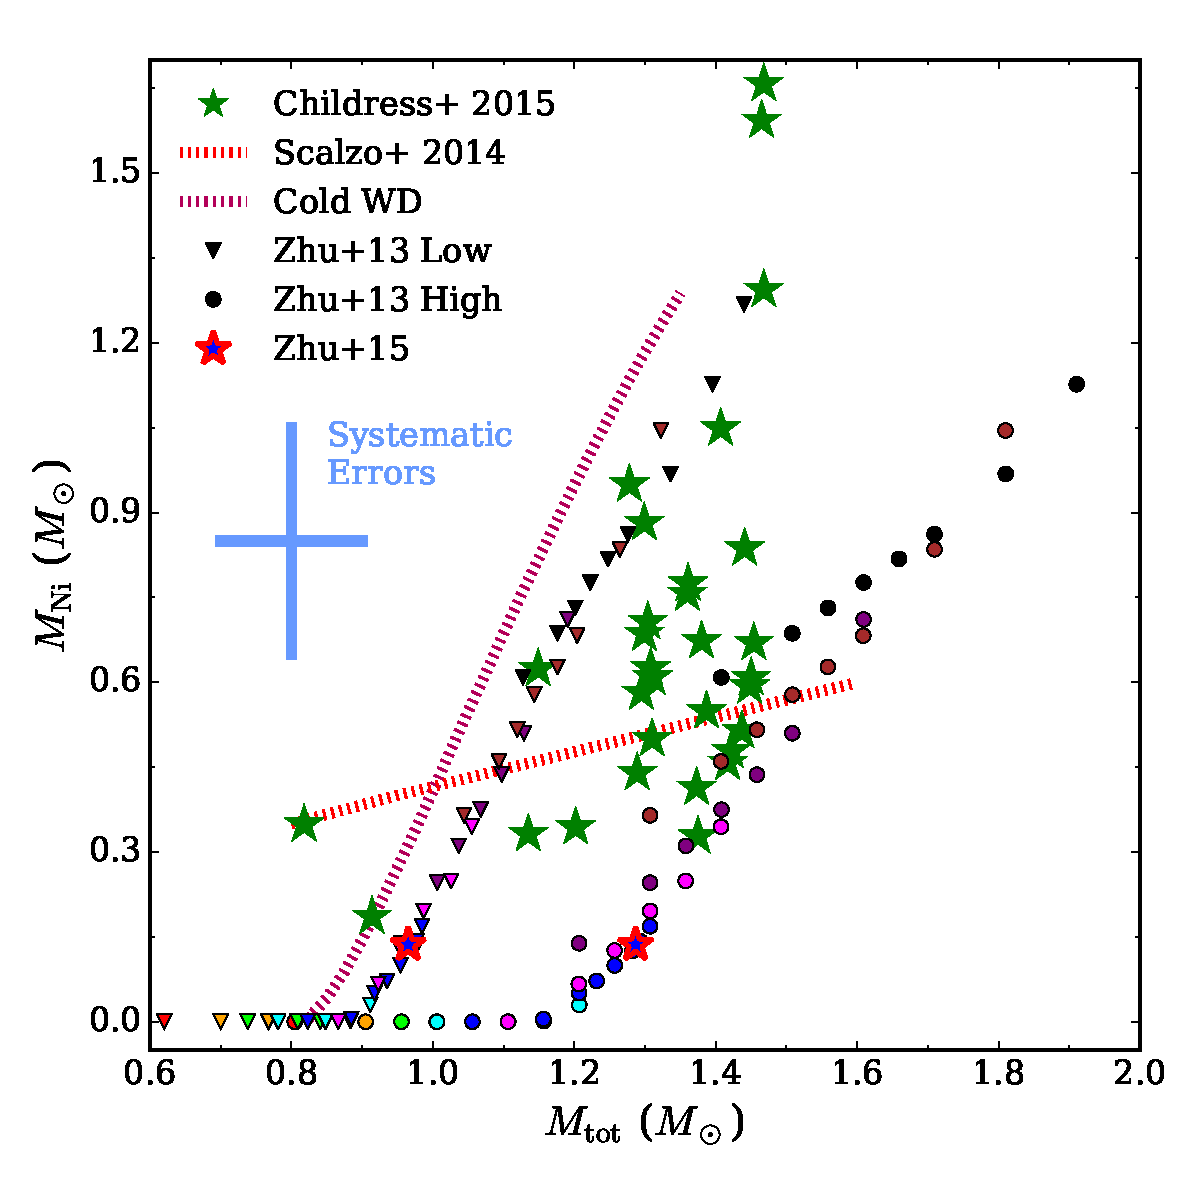
\includegraphics[angle=0,width=0.8\columnwidth]{conclusion/figures/c_MNi.pdf}
\caption{Relationships between total ejected mass \Mtot\ and synthesized \Ni\ mass \MNi\ for the merger remnants of Fig. \ref{fig:c2_pmevolution} if they were to (artificially) experience a pure detonation immediately after their estimated viscous spin-down.  \MNi\ is estimated by the mass of all remnant material with density $\rho>10^7\,\gcc$, $M(\rho>10^7)$.  \Mtot\ is estimated either as the total mass of the remnant (circles) or the mass of its dense core (inverted triangles).  Colors indicate accretor mass, as in Fig. \ref{fig:c2_constacc}.  Also plotted is the estimate for the \arepo\ MHD $0.625 - 0.65\,\Msun$ remnant (Ch. \ref{ch:ch4}; red-blue star).  All other features are as in Fig. \ref{fig:c5_mni}.}
\label{fig:c6_mcmce_mni}
\end{figure}

If powerful magnetic fields can indeed completely suppress convection, this will, at best, prevent any changes in the temperature and density structure of the WD once nuclear burning is lit.  If we assume this is the case, we can estimate the nucleosynthetic yields of our sub-\Mch\ merger remnants.  In Fig. \ref{fig:c6_mcmce_mni}, we plot the total ejected mass \Mtot\ and synthesized \Ni\ mass \MNi\ of all the post-viscous remnants generated by the simple estimate in Sec. \ref{ssec:ch2_viscevo_possiblespindown} -- regardless of whether or not they are predicted to ignite nuclear burning -- if they were to detonate with no change to their structure.  \Mtot\ is assumed to either be the total mass of the merger remnant, or the mass of its dense core following viscous evolution, which brackets the inclusion of the tenuous post-viscous envelope in the explosion.  \MNi\ is estimated by the mass of remnant material with density $\rho>10^7\,\gcc$.  Keeping in mind that our simple estimate tends to overestimate the amount of compression during viscous evolution, particularly for similar-mass mergers (Sec. \ref{sec:c2_postscript}), we see that only mergers with $\Mtot \gtrsim \Msun$ produce more than $\sim0.2\,\Msun$ of \Ni.  Since more realisitic simulations of viscous evolution predict less core compression, and not all remnants will ignite fusion, Fig. \ref{fig:c6_mcmce_mni} estimates the upper limit of \Ni\ produced by the sub-\Mch\ merger channel, and poses a challenge to its viability for producing normal SNe Ia.

\section{What Happens to Sub-\Mch\ Mergers?}

Considering the number of hurdles above, it appears that mergers of two CO WDs whose total mass is substantially below \Mch, including our fiducial $0.625 - 0.65\,\Msun$ merger, are unlikely to produce normal SNe Ia.  The more massive among them may ignite carbon burning, but these will probably become partly non-degenerate and expand before they achieve dynamical burning, eventually transforming their composition to O and Ne before cooling to become massive, highly-magnetized WDs.  Similar-mass super-\Mch\ WDs could perhaps follow \citeal{vkercj10}'s evolutionary channel to ignite highly degenerate nuclear burning and eventually explode: mergers with accretors of $\gtrsim0.8\,\Msun$ create remnants that easily ignite nuclear burning during post-merger evolution and satisfy both the mass and central density constraints suggested by our simmering study.  These systems, however, may have have already exploded in a violent merger (Sec. \ref{ssec:c1_new_typeia}), or shortly after coalescence due to accretion-heating from an $m = 1$ spiral mode \citep{kash+15}.  The minimum masses required for either is not well-known (see \citealt{dan+12, sato+16} for recent estimates for violent mergers), so it remains a task for future parameter-space merger studies to constrain them.
 
\section{Observational Avenues of Exploration}

Finally, we stress the potential of observational work in shedding light on this subject.  Recently revealed properties of the hot DQ population tantalizingly suggest they represent double CO WD merger remnants that did not explode.  Many of their fundamental properties, such as their masses and space density, remain poorly understood, but the Gaia mission will be able to provide parallaxes to help constrain these values \citep{dunl15thesis}.  Future observations will allow us to judge more confidently whether hot DQs are merger remnants.  If they are, the population's properties will serve as an observational check for the theoretical evolutionary scenarios in this work.

It may also be possible to spot merger remnants during their thermal evolution phase described in Sec. \ref{sec:c2_postscript}.  \cite{schw+16} consider the observable properties of their $1.5\,\Msun$ merger remnant, and calculate that it radiates on the order the Eddington luminosity for a $1.5\,\Msun$ star ($\sim10^5\,\Lsun$), and may also generate clouds of dust in its outermost layers, which will be launched as an optically thick wind.  This drives the remnant's photosphere out to $\sim10^{15}\,\mrm{cm}$, with a corresponding photospheric temperature of $\sim500\,\mrm{K}$, as well as possibly RCrB-like variablility of the remnant's luminosity.  \citep{schw+16} notes these features are similar to those of extreme AGB stars (eg. \citealt{blum+06}), and perhaps can be discovered using the same observational techniques.  Since sub-\Mch\ remnants have the same order of magnitude total energy as \Mch\ ones, their observed properties will be similar.

These new observational studies, alongside the theoretical and numerical discussed earlier, may clarify many of the outstanding questions posed throughout this thesis.  With luck, they will also lead to a clearer understanding of the fates of CO WD merger products, and SNe Ia.

%-resummarize all papers
%-don't say what we used to think

%-MRI growth rate in remnant?
%-simulation code does matter for post-merger evolution (hydrodynamic waves, magnetic fields)
%-They note that the luminosity of the nuclear burning zone is almost entirely carried away by neutrino losses (as the burning zone sits at the $\taucc = \taunu$ line), and so the remnant's source of luminosity is the heat from the merger and viscous evolution.

%\section{Does the \citeal{vkercj10} Channel Work?}

%Even if we assume runaways are vertical, the typical spun-down remnant still doesn't get to 1e7 gcc!

%%This result poses a problem for the \citeal{vkercj10} sub-\Mch\ merger channel.  \cite{shen+12} finds further compression could occur during the subsequent \textit{thermal} evolution of the remnant over $\gtrsim10^4\,\mrm{yr}$, which may allow more remnants to reach higher central density and enclose more mass within their cores.  Whether central burning could still begin is uncertain, however, since thermal diffusion and neutrino-driven cooling may favor off-center carbon ignition, or simply net cooling, even for those post-viscous remnants that are initially $\gtrsim5\times10^8\,\mrm{K}$ at their center.  Moreover, remnants, with radiation-dominated and highly magnetized carbon atmospheres, will likely drive strong outflows during their thermal evolution, further complicating predictions.  We note one advantage for delaying the explosion to during thermal evolution is the removal of the ``clutter'' of the $\gtrsim0.1\,\Msun$ hot envelope surrounding the core and extending out to $\gtrsim10^{11}\,\mrm{cm}$ \citep{shen+12}.  This imparts signatures onto the explosion not seen in ordinary SNe Ia, such as a double-peaked light curve from the shock cooling of the envelope, excess blue and UV emission prior to peak light, and a slow-decaying light curve near peak light \citep{frye+10,levasg15,pirom15}.  While \cite{shen+12}'s simulation suggests thermal evolution will do little to alter the overall structure of the envelope \citep{pirom15}, it does not account for mass loss due to winds.  These will significantly alter the size and structure of the envelope, perhaps mitigating its effects on any eventual explosion.  Meanwhile, material ejected from the remnant (both during its viscous and subsequent thermal phases) moving at the escape velocity will approach $\sim10^{17}\,\mrm{cm}$ after $\sim10^4\,\mrm{yr}$.  Interaction between this material and light from the supernova could explain \citep{shen+12, ji+13} observations of SN Ia-CSM interactions such as time-variable NaID lines (eg. \citealt{pata+07, simo+09}).

%% Magnetic coupling between the outflow and the remnant will aid in its spindown and possibly generate non-local heating through magnetic resistivity.

%Is the classic Mch DD channel even possible?

%-
%-





%\section{Observable Counterparts to Mergers}

%\section{The Evolution and Appearance of Quiescent Merger Remnants}

%% Shen+12 gives the escape velocity at 10^13 cm as 60 km/s.  Given 10^4 years of evolution, this wind could transport material to 10^18 cm, possibly explaining the variable sodium emission.

%\section{The Influence of Merger Remnants Properties on Potential Explosions}

%If sub-\Mch\ CO WD merger remnants indeed trigger thermonuclear detonations following post-merger viscous evolution, will these explosions resemble SNe Ia?  As noted in the introduction, SNe Ia observations and radiative transfer models for explosions are now sophisticated enough to distinguish fine details between different progenitors.  This question has been taken up by a number of theorists \citep{frye+10, shen+12}  Shen+12 conclusions!

%\cite{frye+10} and \cite{rask+14} do simulations

%\begin{itemize}
%	\item What are the mass loss rates of non-explosive mergers due to carbon dust superwind?  can we estimate?  could it possibly lead to Kepler's 0.6Msun oxygen WD? Shen+12 (Just under Eqn. 7) note that mass loss in radiation-dominated H/He-deficient envelopes is poor. %http://adsabs.harvard.edu/abs/2016Sci...352...67K
%	\item Near-eddington carbon burning star?  See Sec. 4 paragraph 1 of Shen+12.
%	\item Discussion with Marten: while we can't rule out further compression leading to nuclear burning during the thermal evolution phase, a combination of magnetically and Eddington-launched outflows will make the surroundings very messy - write more about this in SN Ia appearance stuff.
%	\item Importance of Ia-CSM stuff?  Shen+12 and Ji+13 (Sec. 2.2.3) have extensive sections on it.
%	\item Ji+13 has a mean magnetic field of 2e8 G; what does our simulation have?  They also (bottom of pg 7) give a quick estimate for magnetic lifetime.
%	\item What's the difference between a ring of material at $10^{13}$ cm and a continuous envelope that ends at the same radius?  Does one resemble Ia-CSM interaction, but the other lead to Fryer+10 or Piro+15 early time brightening?
%	\item Even super chandra DD systems will be much less dense than their WD binary progenitors - consequences for explosions?
%\end{itemize}



%\section{Avenues for Future Exploration}


%\subsection{Future Simulations of Mergers and Post-Merger Evolution}

%Do we need to simulate more merging WDs, especially using novel magnetohydrodynamic schemes?  Ch. STUFF suggests that the hydrodynamics up to coalescence and overall remnant properties do not substantively change when transitioning from simulating with a traditional variant of SPH to doing so with a modern moving mesh code, and getting the initial conditions (eg. synchronization, accurate tidal bulges for the onset of mass transfer) right is likely to be more important.  We await results from the the Eulerian grid WD merger simulations of \citep{katz+16} for further confirmation.

%What does require further work is the magnetic evolution during the merger, as well as the early phase of post-merger evolution and further magnetic field growth following coalescence.  The former has been insufficiently investigated with the latest generation of MHD codes, which may end up predicting very different field configurations (and possibly energies) than our exploration of the problem with \arepo.  The latter, however, is not only also poorly explored (only one group has conducted a full MHD simulation!) but essential to better understanding post-merger evolution.  This regime is particularly challenging for codes, since it requires the code minimize numerical hydrodynamic and magnetic viscosity (traditionally problematic for SPH codes) while maintaining conservative quantities -- particularly angular momentum -- over hundreds of dynamical times (traditionally difficult for grid codes).  Moreover, the problem is stiff, since evolution occurs both on a dynamical (with spiral waves) and viscous timescale, and thus quite computationally intensive.  We note the recent introduction of two codes: duffel's and hopkins', that could potentially bridge the gap.

%Arepo MHD doesn't do a good job of conserving angular momentum - balance plot shows it spurious gains it.  May be due to divergence cleaning (hopkins 16)


%Simulations of detonations within violent mergers (eg. \ref{pakm+10, bull+16, krom+16}) or mergers shortly after coalescence \citep{rask+14,vros+15}, do not reproduce the light curves and spectra of SNe Ia.  

%OUR REMNANTS AREN'T RADIATION DOMINATED.  Prad/Pion \propto T^3/\rho \propto \rho in adiabatic envelopes; we're in general much colder for any given density than Shen+12, so in fact we don't have radiation dominated envelopes, but we still have extended ones!

%Shen+16 is important, since nuclear burning energy doesn't get to exterior before 1e4 years are up, so non-burning remnants will look similar!

%It may also be possible to spot merger remnants during their thermal evolution phase described in Sec. \ref{sec:c2_postscript}.  \cite{schw+16} consider in depth the observable properties of their $\1.5\,\Msun$ merger remnant undergoing carbon and neon burning.  They note that the luminosity of the nuclear burning zone is almost entirely carried away by neutrino losses (as the burning zone sits at the $\taucc = \taunu$ line), and so the remnant's source of luminosity is the heat from the merger and viscous evolution.  Since sub-\Mch\ remnants have the same order of magnitude total energy as \Mch\ ones, their observed properties will be similar.  \cite{schw+16} find that, with an envelope and a radiation-dominated hot atmosphere of $10^{12}-10^{13}\,\mrm{cm}$, the remnant initially radiates of order the Eddington luminosity for a $1.5\,\Msun$ star ($\sim10^5\,\Lsun$) and has a photospheric temperature ranging from $4000 - 10^5\,\mrm{K}$.  The remnant may also generate clouds of dust in their outermost layers, which will then be launched as an optically thick wind, driving the remnant's photosphere out to $\sim10^{15}\,\mrm{cm}$, with corresponding photospheric temperatures of $\sim500\,\mrm{K}$, and lead to RCrB-like variablility in the remnant's luminosity.  \citep{schw+16} notes these features are similar to those of extreme AGB stars (eg. \citealt{blum+06}).

%krom+16 http://adsabs.harvard.edu/doi/10.1093/mnras/stw962
%bull+16 http://adsabs.harvard.edu/abs/2016MNRAS.455.1060B
%vros+15 http://adsabs.harvard.edu/abs/2015arXiv151004286V
%papi+15 http://adsabs.harvard.edu/abs/2015MNRAS.449..942P
%pirom15 http://adsabs.harvard.edu/abs/2015arXiv151203442P

